\documentclass[11pt]{article}
\usepackage[margin=2.3cm]{geometry}
\usepackage{amsmath}
\usepackage{tikz}
\usetikzlibrary{arrows.meta,positioning,fit,backgrounds,shapes.multipart,calc,decorations.pathreplacing}
\usepackage{forest}
\usepackage{listings}
\usepackage{xcolor}
\usepackage{booktabs}
\usepackage{longtable}
\usepackage{parskip}
\usepackage{hyperref}
\usepackage{titlesec}
\usepackage{enumitem}
\usepackage{fancyhdr}
\usepackage{tcolorbox}
\tcbuselibrary{skins,breakable}

\hypersetup{colorlinks=true,linkcolor=blue!50!black,urlcolor=blue!50!black,citecolor=blue!50!black}
\definecolor{codebg}{RGB}{245,245,245}
\definecolor{accent}{RGB}{20,80,150}
\definecolor{defbox}{RGB}{235,242,250}

\lstset{
  basicstyle=\ttfamily\small,
  backgroundcolor=\color{codebg},
  breaklines=true,
  frame=single,
  framerule=0.3pt,
  rulecolor=\color{gray!40},
  columns=fullflexible,
  keywordstyle=\color{accent}\bfseries,
  commentstyle=\color{gray},
  showstringspaces=false,
  xleftmargin=2pt, xrightmargin=2pt,
}

\titleformat{\section}{\large\bfseries\color{accent}}{\thesection}{0.6em}{}
\titleformat{\subsection}{\normalsize\bfseries}{\thesubsection}{0.6em}{}

\pagestyle{fancy}
\fancyhf{}
\fancyhead[L]{\small agent-runtime --- Deep Dive}
\fancyhead[R]{\small\thepage}
\renewcommand{\headrulewidth}{0.3pt}

\newtcolorbox{defterm}[1]{colback=defbox,colframe=accent!60!black,title={\textbf{Term: #1}},fonttitle=\small\bfseries,coltitle=white,boxrule=0.4pt,left=6pt,right=6pt,top=3pt,bottom=3pt,breakable}

\newcommand{\code}[1]{\texttt{\small #1}}
\sloppy
\emergencystretch=2.5em

\title{\vspace{-1.5cm}\textbf{\Huge agent-runtime}\\[0.3cm]\Large Deep Dive: an event-sourced runtime for tool-using LLM agents}
\author{Explainer generated for the project owner \\ \small A beginner-safe, exhaustive technical walkthrough of the actual codebase}
\date{}

\begin{document}
\maketitle
\thispagestyle{empty}

\begin{tcolorbox}[colback=yellow!10,colframe=yellow!50!black,title=How to read this document,fonttitle=\bfseries]
This document explains \textbf{exactly} what is implemented in the \code{agent-runtime}
project folder, as of the code and tests present at the time of writing. Every claim
traces to a specific file. Technical terms are defined the first time they appear, in a
boxed callout like this one. Nothing here is invented: where the project's own README
states an honest limitation (e.g. ``no live API calls were made''), this document
repeats it rather than smoothing it over.
\end{tcolorbox}

\tableofcontents
\newpage

% ============================================================
\section{What this project is}
% ============================================================

\textbf{agent-runtime} is a Python library and command-line tool for running
\emph{LLM agents} --- programs that use a large language model (LLM) to decide, in a
loop, which actions to take next --- with the operational machinery that a bare
``call the model, run a tool, repeat'' loop leaves out: a durable record of every run,
the ability to replay a run exactly, safe recovery from a crash mid-run, a human
approval step before anything with a side effect happens, deliberately injected
failures to prove the system degrades safely, and a suite of scripted regression tests
that catch behavior changes when the underlying model changes.

\begin{defterm}{LLM agent}
A program where a large language model is asked, in a loop, ``given what has
happened so far, what should happen next?'' The model's answer is either a final
text answer, or a request to call one or more \emph{tools} (functions the program
exposes, such as ``read this file'' or ``send this HTTP request''). The program
executes the requested tool(s), feeds the result back to the model, and asks again.
This project implements exactly that loop in \code{src/agent\_runtime/runtime.py}.
\end{defterm}

\subsection*{Why it exists (the project's own framing)}
The project's README states its thesis directly: the agent loop itself is a small
amount of code, but what makes an agent \emph{deployable} is everything around it ---
knowing exactly what happened in a specific run, being able to reproduce that run,
knowing whether the agent took an action (e.g.\ emailed a customer) before a human
approved it, and knowing whether a new model version still passes the flows that used
to work. The project's design response to all of this is a single idea, applied
consistently: \textbf{every run is an append-only log of events, and every feature is
a function computed from that log.}

\begin{defterm}{Event sourcing}
A design pattern where, instead of storing ``the current state'' of something and
overwriting it as things change, you store every state-changing event as an immutable,
ordered record, and compute ``current state'' on demand by replaying those events from
the start. Because the log never loses information, you can always recompute the past,
replay it, or audit it. This project's central and only source of truth is such a log,
one table row per event.
\end{defterm}

% ============================================================
\section{Architecture at a glance}
% ============================================================

\begin{center}
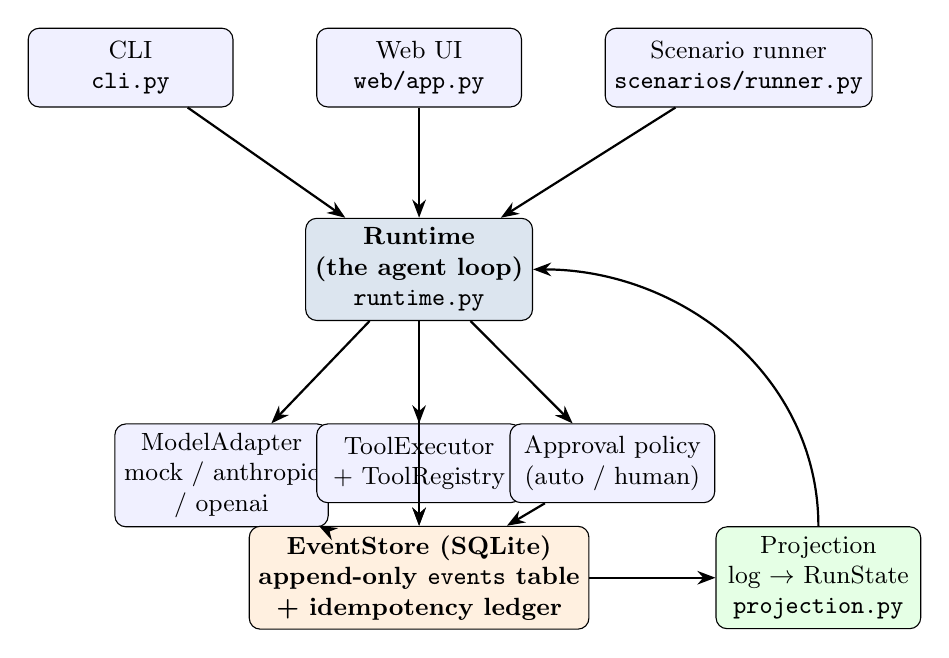
\begin{tikzpicture}[
  box/.style={draw, rounded corners, fill=blue!6, minimum height=1cm, minimum width=2.6cm, align=center, font=\small},
  core/.style={box, fill=accent!15, font=\small\bfseries},
  store/.style={draw, fill=orange!12, minimum height=1.1cm, minimum width=3.6cm, align=center, font=\small\bfseries, rounded corners},
  arr/.style={-{Stealth[length=2.3mm]}, thick},
  node distance=1.05cm and 1.05cm
]
  \node[box] (cli) {CLI\\ \code{cli.py}};
  \node[box, right=of cli] (web) {Web UI\\ \code{web/app.py}};
  \node[box, right=of web] (scen) {Scenario runner\\ \code{scenarios/runner.py}};

  \node[core, below=1.4cm of web] (rt) {Runtime\\ (the agent loop)\\ \code{runtime.py}};

  \node[box, below left=1.3cm and -0.3cm of rt] (adapter) {ModelAdapter\\ mock / anthropic\\ / openai};
  \node[box, below=1.3cm of rt] (exec) {ToolExecutor\\ + ToolRegistry};
  \node[box, below right=1.3cm and -0.3cm of rt] (appr) {Approval policy\\ (auto / human)};

  \node[store, below=2.6cm of rt] (store) {EventStore (SQLite)\\ append-only \code{events} table\\ + idempotency ledger};

  \node[box, right=1.6cm of store, fill=green!10] (proj) {Projection\\ log $\rightarrow$ RunState\\ \code{projection.py}};

  \draw[arr] (cli) -- (rt);
  \draw[arr] (web) -- (rt);
  \draw[arr] (scen) -- (rt);
  \draw[arr] (rt) -- (adapter);
  \draw[arr] (rt) -- (exec);
  \draw[arr] (rt) -- (appr);
  \draw[arr] (adapter) -- (store);
  \draw[arr] (exec) -- (store);
  \draw[arr] (appr) -- (store);
  \draw[arr] (rt) -- (store);
  \draw[arr] (store) -- (proj);
  \draw[arr] (proj.north) to[out=90,in=0] (rt.east);
\end{tikzpicture}
\end{center}

Every arrow into the SQLite store is an \emph{append}: the codebase contains no
UPDATE or DELETE against the \code{events} table (confirmed by reading
\code{store.py} in full --- the schema and every SQL statement in that file are
\code{INSERT} or \code{SELECT}). Every arrow out of the store goes through
\code{projection.py}, which is the \emph{only} module that interprets what a
sequence of events means. The CLI, the web UI, the replay comparator and the
scenario-test assertions all call the same \code{project()} function, so they
cannot disagree about the state of a run.

\begin{defterm}{SQLite}
A small, file-based relational database engine that needs no separate server process
--- the whole database is one file on disk. This project uses it as the single
persistent store for every run's event log.
\end{defterm}

% ============================================================
\section{The event log: the one idea everything is built on}
% ============================================================

\subsection{The \code{events} table}
From \code{store.py}, the schema actually created is:

\begin{lstlisting}[language=SQL]
CREATE TABLE events (
    run_id  TEXT    NOT NULL,
    seq     INTEGER NOT NULL,
    type    TEXT    NOT NULL,
    ts      REAL    NOT NULL,
    payload TEXT    NOT NULL,   -- JSON blob
    PRIMARY KEY (run_id, seq)
);
CREATE TABLE executions (          -- the idempotency ledger, see Sec. 6
    idem_key TEXT PRIMARY KEY,
    run_id   TEXT NOT NULL,
    result   TEXT NOT NULL,
    ts       REAL NOT NULL
);
\end{lstlisting}

\begin{defterm}{Primary key / append-only}
A \emph{primary key} is a column (or combination of columns) that must be unique per
row and is used to look rows up quickly. Here the primary key is
\code{(run\_id, seq)}: for a given run, each sequence number can be claimed only
once. \code{EventStore.append()} reads \code{MAX(seq)+1} for the run, tries to
insert, and retries (up to 5 times) if another writer raced it to the same number
--- this is what makes two processes appending to the same run safe without needing
a lock: SQLite's uniqueness constraint on the primary key rejects the loser, who then
just re-reads the new max and tries again.
\end{defterm}

\subsection{Event types}
\code{events.py} defines twelve event type constants (grouped here in the order a
typical successful run emits them):

\begin{center}
\small
\begin{tabular}{@{}p{3.6cm}p{9.8cm}@{}}
\toprule
\textbf{Event type} & \textbf{Payload highlights (from \code{projection.py} / \code{runtime.py})} \\
\midrule
\code{run\_created} & agent name, the user's request text, and free-form \code{meta} (workspace path, which adapter, scenario file if any) \\
\code{model\_requested} & a call number, and a \emph{digest} (short hash) and count of the messages about to be sent --- not the messages themselves \\
\code{model\_responded} & the parsed turn (text and/or tool calls), token usage, model name; or \code{malformed: true} with the raw unparseable text \\
\code{model\_error} & a transport/provider failure for one attempt (e.g.\ simulated HTTP 500) \\
\code{tool\_requested} & call id, tool name, arguments, and whether the tool is a side-effecting one \\
\code{tool\_approved} / \code{tool\_denied} & who approved/denied, and the deny reason if any \\
\code{tool\_executed} / \code{tool\_failed} & the tool's result or error, and how many attempts it took \\
\code{checkpoint} & how many model calls and resolved tool calls have happened so far (a periodic marker, not needed for correctness --- see Sec.\ 4) \\
\code{run\_finished} / \code{run\_failed} & the model's final answer text, or a machine-readable failure cause string \\
\bottomrule
\end{tabular}
\end{center}

\begin{defterm}{Digest / hash}
A short, fixed-length string computed from a larger piece of data such that the same
input always produces the same digest, and different inputs almost never produce the
same one. This project uses SHA-256 (a standard cryptographic hash function) truncated
to 16 hex characters purely as a fingerprint of the outgoing message list --- it is
not meant to be secret, just a compact ``was this the same request'' marker
(\code{runtime.\_digest}).
\end{defterm}

\subsection{Canonical encoding, for exact comparison}
Every \code{Event} has a \code{canonical()} method that JSON-encodes it with sorted
keys and no extra whitespace:
\begin{lstlisting}[language=Python]
json.dumps(body, sort_keys=True, separators=(",", ":"))
\end{lstlisting}
Two events that mean the same thing always produce the exact same string. This is
what lets \emph{replay} (Sec.\ 7) claim ``byte-identical'' rather than
``looks about right.''

% ============================================================
\section{The agent loop: \code{Runtime.drive()}}
% ============================================================

\code{runtime.py}'s \code{Runtime} class is the heart of the project. Its
\code{drive(run\_id)} method is, in the project's own words, ``a fixed-point
iteration over the log'': it keeps re-deriving what to do next purely from the
current event log, until the run reaches a terminal state.

\begin{defterm}{Fixed-point iteration}
A loop that repeatedly applies the same rule to its own output until the output stops
changing (or a stated exit condition is hit). Here, ``derive the current state from
the log, decide the single next thing to do, append it, repeat'' is applied
identically whether this is the very first iteration of a brand-new run, the
continuation of a run just approved by a human, or the resumption of a run that
crashed a minute ago. There is exactly one code path, not three.
\end{defterm}

\begin{center}
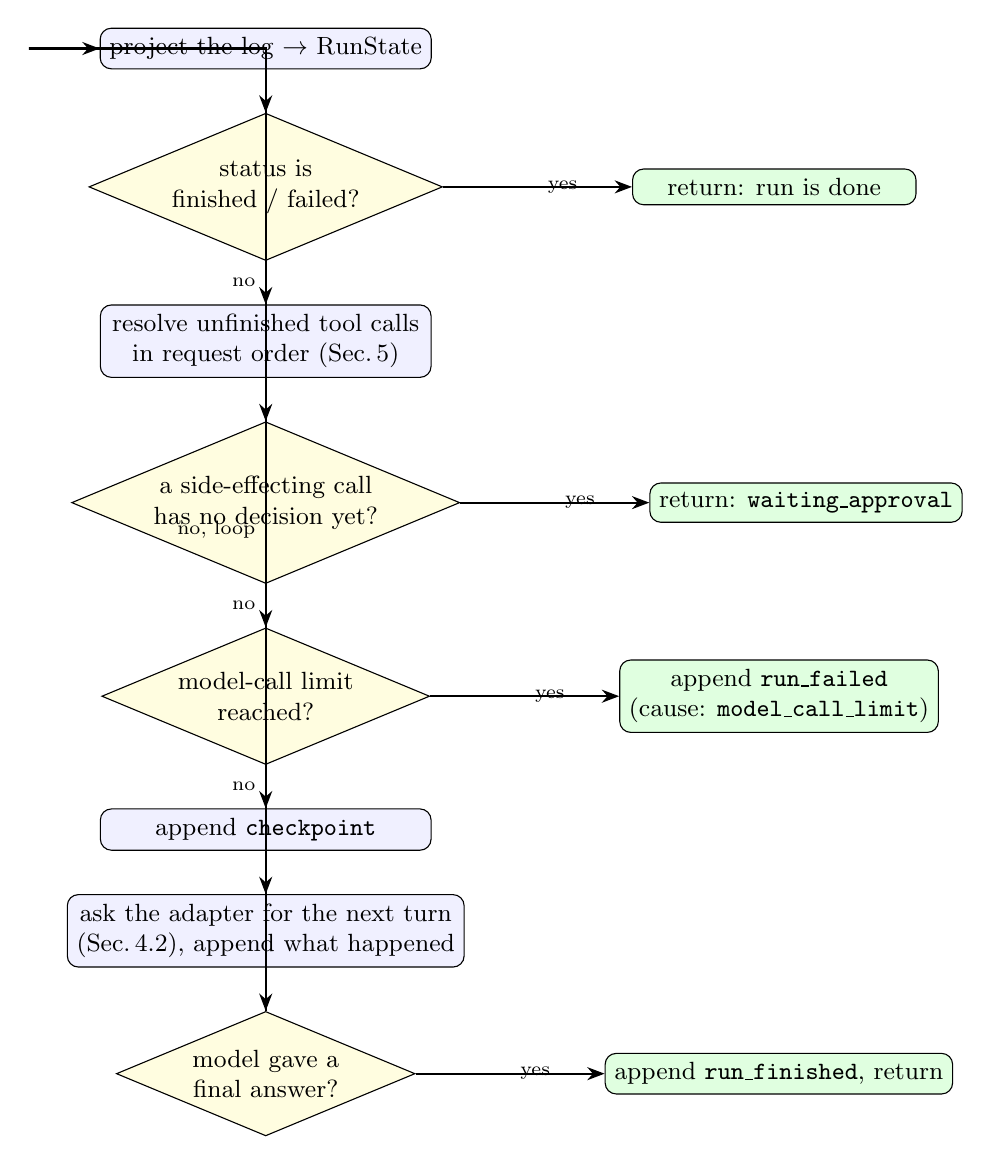
\begin{tikzpicture}[
  node distance=0.55cm and 1.2cm,
  d/.style={draw, diamond, aspect=2.4, fill=yellow!12, align=center, font=\small, inner sep=2pt},
  s/.style={draw, rounded corners, fill=blue!6, align=center, font=\small, minimum width=4.2cm},
  t/.style={draw, rounded corners, fill=green!12, align=center, font=\small, minimum width=3.6cm},
  arr/.style={-{Stealth[length=2.2mm]}, thick}
]
  \node[s] (start) {project the log $\rightarrow$ RunState};
  \node[d, below=of start] (terminal) {status is\\finished / failed?};
  \node[t, right=2.4cm of terminal] (stop1) {return: run is done};
  \node[s, below=of terminal] (resolve) {resolve unfinished tool calls\\ in request order (Sec.\,5)};
  \node[d, below=of resolve] (paused) {a side-effecting call\\ has no decision yet?};
  \node[t, right=2.4cm of paused] (stop2) {return: \code{waiting\_approval}};
  \node[d, below=of paused] (limit) {model-call limit\\ reached?};
  \node[t, right=2.4cm of limit] (stop3) {append \code{run\_failed}\\ (cause: \code{model\_call\_limit})};
  \node[s, below=of limit] (checkpoint) {append \code{checkpoint}};
  \node[s, below=of checkpoint] (model) {ask the adapter for the next turn\\ (Sec.\,4.2), append what happened};
  \node[d, below=of model] (final) {model gave a\\ final answer?};
  \node[t, right=2.4cm of final] (stop4) {append \code{run\_finished}, return};

  \draw[arr] (start) -- (terminal);
  \draw[arr] (terminal) -- node[right,font=\scriptsize]{yes} (stop1);
  \draw[arr] (terminal) -- node[left,font=\scriptsize]{no} (resolve);
  \draw[arr] (resolve) -- (paused);
  \draw[arr] (paused) -- node[right,font=\scriptsize]{yes} (stop2);
  \draw[arr] (paused) -- node[left,font=\scriptsize]{no} (limit);
  \draw[arr] (limit) -- node[right,font=\scriptsize]{yes} (stop3);
  \draw[arr] (limit) -- node[left,font=\scriptsize]{no} (checkpoint);
  \draw[arr] (checkpoint) -- (model);
  \draw[arr] (model) -- (final);
  \draw[arr] (final) -- node[right,font=\scriptsize]{yes} (stop4);
  \draw[arr] (final) |- node[near start,left,font=\scriptsize]{no, loop} ($(start.west)+(-0.9,0)$) -- (start.west);
\end{tikzpicture}
\end{center}

\subsection{Resolving tool calls (step ``resolve unfinished tool calls'')}
\code{RunState.unfinished\_calls()} returns every requested tool call that is still
\code{requested} or \code{approved} (i.e.\ not yet executed/denied/failed), in the
order they were requested. For each:
\begin{itemize}[nosep]
  \item If it is \textbf{not} a side-effecting call, or it was already approved, it
  executes immediately (Sec.\,6).
  \item If it \textbf{is} side-effecting and undecided, the \emph{approval policy}
  (a plain function taking the call and returning approve/deny/\code{None}) is
  consulted. \code{None} means ``ask a human'' --- the loop returns
  \code{waiting\_approval} right there, without touching later calls.
\end{itemize}

\begin{defterm}{Side effect}
An action with a lasting, observable consequence outside the running program ---
writing a file, updating a spreadsheet, adding a calendar entry, drafting an email.
Contrast with a \emph{read-only} action (reading a file, listing a directory), which
can be safely retried or re-run because it changes nothing. Every tool in this
project declares a boolean \code{side\_effect} flag (\code{tools/registry.py}); only
side-effecting tools are gated behind human approval.
\end{defterm}

\subsection{Asking the model (step ``ask the adapter'')}
\code{\_model\_step()} rebuilds the conversation from the log via
\code{build\_messages()} (Sec.\,5), appends \code{model\_requested}, then calls
\code{adapter.complete(messages, tool\_specs)}. Three outcomes are handled:
\begin{enumerate}[nosep]
  \item \textbf{Transport/provider failure} (\code{AdapterError}): appends
  \code{model\_error} and, if retries remain (default 2), sleeps
  \code{0.5s $\times 2^{\text{attempt}}$} (exponential backoff) before retrying.
  If retries are exhausted, appends \code{run\_failed} with cause
  \code{adapter\_error: retries exhausted}.
  \item \textbf{Unparseable output} (\code{MalformedOutputError}): appends
  \code{model\_responded} with \code{malformed: true} and the raw text. If this is
  more than \code{max\_malformed} (default 2) malformed responses total for the run,
  the run fails with cause \code{malformed\_model\_output: \dots}; otherwise the loop
  returns \code{False} (not done) and the next iteration's \code{build\_messages()}
  will include a corrective message telling the model to try again (Sec.\,5).
  \item \textbf{A parsed turn}: appended as \code{model\_responded}. If the turn has
  no tool calls (\code{ModelTurn.is\_final}), it is the final answer and
  \code{run\_finished} is appended. Otherwise, every requested tool call becomes a
  \code{tool\_requested} event, tagging each with whether it is side-effecting
  (looked up from the tool registry).
\end{enumerate}

\begin{defterm}{Exponential backoff}
A retry strategy where each successive retry waits longer than the last (here,
doubling: 0.5s, 1s, 2s, \dots), so a struggling remote service is not immediately
hit again at full speed.
\end{defterm}

\subsection{Checkpoints}
Before each model call (except the very first), the loop appends a \code{checkpoint}
event recording how many model calls and resolved tool calls have happened.
Read literally in the code, a checkpoint is \emph{not} required for the loop's
correctness --- everything can already be recomputed from the rest of the log --- it
exists as a cheap, explicit marker of progress useful for a human skimming
\code{agentrun runs show}.

% ============================================================
\section{Rebuilding a conversation from the log}
% ============================================================

\code{projection.build\_messages(state, system\_prompt)} in \code{projection.py}
turns the event log into the list of messages a model API expects: a system prompt,
the user's original request, then one message per subsequent turn or observation ---
walking the log in order and translating:

\begin{center}
\small
\begin{tabular}{@{}p{4.2cm}p{9.2cm}@{}}
\toprule
\textbf{Log event} & \textbf{Message produced} \\
\midrule
\code{model\_responded} (normal) & an \code{assistant} message: the turn's text, plus \code{tool\_calls} if any \\
\code{model\_responded} (malformed) & a \code{user} message: ``Your previous output could not be parsed. Reply with either tool calls or a final answer.'' --- this is the corrective nudge mentioned in Sec.\,4.2 \\
\code{tool\_executed} & a \code{tool} message carrying the result \\
\code{tool\_failed} & a \code{tool} message: \code{\{"error": \dots\}} \\
\code{tool\_denied} & a \code{tool} message: \code{\{"denied": true, "reason": \dots\}} --- this is literally how ``the operator said no'' becomes something the model can react to \\
\bottomrule
\end{tabular}
\end{center}

Because this is a pure function of the log, a run resumed after a crash sends the
model \emph{exactly} the same messages an uninterrupted run would have sent at that
point --- there is no separate ``resume state'' to keep in sync.

Each concrete adapter (Sec.\,8) then translates this provider-neutral list into the
wire format its specific API expects (Anthropic content blocks, or OpenAI chat
messages with a \code{tool\_call\_id}).

% ============================================================
\section{Idempotency and the crash window}
% ============================================================

\begin{defterm}{Idempotency}
An operation is \emph{idempotent} if doing it twice has the same effect as doing it
once. Re-reading a file is naturally idempotent. Sending a reminder email is not ---
sending it twice annoys the customer twice. This project makes tool execution
idempotent \emph{per run} by remembering that it already ran, so a retried/resumed
run does not repeat it.
\end{defterm}

\code{tools/executor.py}'s \code{ToolExecutor.execute()} derives a key from
\code{(run\_id, seq of the tool\_requested event)}:
\begin{lstlisting}[language=Python]
def idempotency_key(run_id, requested_seq):
    return hashlib.sha256(f"{run_id}:{requested_seq}".encode()).hexdigest()[:32]
\end{lstlisting}
Both inputs are identical whether this is the first attempt or a resume after crash,
so the key is stable. The write order is deliberate:

\begin{center}
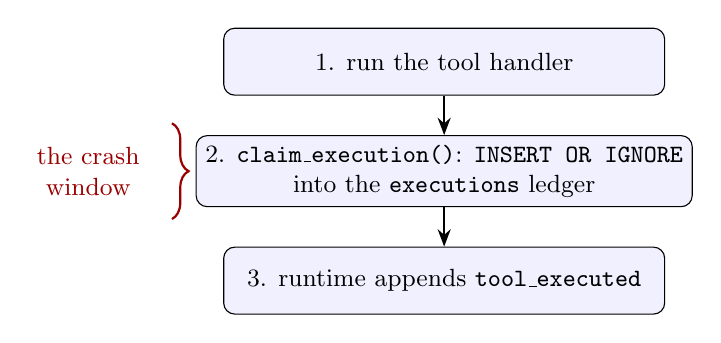
\begin{tikzpicture}[
  node distance=0.5cm and 0.4cm,
  s/.style={draw, rounded corners, fill=blue!6, align=center, font=\small, minimum width=5.6cm, minimum height=0.85cm},
  arr/.style={-{Stealth[length=2.2mm]}, thick}
]
  \node[s] (h) {1. run the tool handler};
  \node[s, below=of h] (l) {2. \code{claim\_execution()}: \code{INSERT OR IGNORE}\\ into the \code{executions} ledger};
  \node[s, below=of l] (a) {3. runtime appends \code{tool\_executed}};
  \draw[arr] (h) -- (l);
  \draw[arr] (l) -- (a);
  \draw[decorate, decoration={brace, amplitude=6pt}, thick, red!60!black]
    ($(l.north west)+(-0.3,0.15)$) -- ($(l.south west)+(-0.3,-0.15)$)
    node[midway, left=8pt, align=center, font=\small, color=red!60!black]
    {the crash\\ window};
\end{tikzpicture}
\end{center}

If the process dies between step 2 and step 3 --- the worst possible instant, after
the real-world side effect already happened but before the log says so --- a
subsequent resume calls \code{execute()} again with the \emph{same} key, finds a
row already in the \code{executions} ledger (via \code{get\_execution()}), and
returns that recorded result immediately without touching the handler again. The
runtime then appends \code{tool\_executed} with an extra \code{replayed: true} flag,
so the log itself records that this particular execution didn't actually re-run.
\code{tests/test\_resume.py} exercises exactly this crash point (via a small executor
wrapper that raises \emph{after} the handler has run but before the ledger write
would normally be reached) and asserts a side-effect counter --- e.g.\ number of
\code{.eml} draft files written --- stays at 1.

The README calls out one honest limitation here: because
\code{concurrent.futures} timeouts (Sec.\,9) abandon a worker thread rather than
kill it, a genuinely hung tool leaks a thread per retried attempt; this is
documented as a known gap, not silently hidden.

% ============================================================
\section{Deterministic replay}
% ============================================================

\begin{defterm}{Replay}
Re-executing a program's logic using only what was recorded about a previous
execution, with no live external calls, and checking that the result matches what
was recorded. This project's replay does not call any model, run any real tool
handler, or touch the network; every input the loop would normally fetch live
(the next model turn, a tool's outcome, an approval decision, even the wall-clock
time) is instead served from the four ``recorded stand-ins'' below.
\end{defterm}

\code{replay.py}'s \code{replay\_run()} builds four objects, each substituting for a
real dependency, all reading from the same source event list:

\begin{center}
\small
\begin{tabular}{@{}p{3.6cm}p{4.6cm}p{4.6cm}@{}}
\toprule
\textbf{Stand-in} & \textbf{Replaces} & \textbf{Replays from} \\
\midrule
\code{\_RecordedClock} & \code{time.time} & the exact \code{ts} of each original event, in order \\
\code{\_RecordedAdapter} & the live \code{ModelAdapter} & each \code{model\_error} or \code{model\_responded} event, in order, re-raising errors/malformed outputs exactly as before \\
\code{\_RecordedExecutor} & \code{ToolExecutor} & the \code{tool\_executed}/\code{tool\_failed} outcome recorded for each \code{tool\_requested}'s sequence number \\
\code{\_RecordedApprovals} & the live approval policy & the \code{tool\_approved}/\code{tool\_denied} decision recorded per call id \\
\bottomrule
\end{tabular}
\end{center}

The real, unmodified \code{Runtime} then drives the loop exactly as normal, writing
to a fresh run id (\code{<original>-replay-<random>}) in the \emph{same} database
file. Afterwards, \code{canonical\_log()} (Sec.\,3.3) encodes both the original and
the replayed event lists, and they are compared. If they differ, the code walks both
lists in lock-step and reports the sequence number of the first event whose canonical
form differs --- so a divergence is reported as ``first differing event N,'' not just
``it's different somewhere.''

\code{agentrun replay <run-id> --until <seq>} truncates the source log to events up
to \code{seq} before replaying, giving a snapshot of what the run's state looked
like at that exact point --- useful for stepping through a failure. Truncating the
log can leave the replayed loop asking for a model turn or clock tick that was never
recorded; rather than special-casing this, the recorded stand-ins simply raise when
exhausted, and \code{replay\_run()} catches that \code{RuntimeError} and treats
whatever was appended up to then as the answer.

This doubles as a regression tripwire for the runtime's own code: if a future change
to the loop alters the exact sequence of events it produces, replaying an
\emph{old, previously-recorded} run will now diverge from its own recorded log and
say exactly where.

% ============================================================
\section{Failure injection}
% ============================================================

\begin{defterm}{Fault injection}
Deliberately making a system behave as if something went wrong (a timeout, a
malformed response, a server error) in a controlled test, to verify the system
handles that failure the way it's supposed to, instead of only ever testing the
happy path.
\end{defterm}

\code{faults.py} defines \code{FaultPlan}, a plain data class (loadable straight
from a scenario's YAML \code{faults:} block) with two kinds of entries:

\begin{lstlisting}
faults:
  model:
    - {at_call: 2, kind: malformed}      # or kind: adapter_500
  tools:
    read_file:
      - {at_attempt: 1, kind: exception, message: "disk error"}
      - {at_attempt: 2, kind: timeout}
\end{lstlisting}

\code{model\_fault(call\_number)} is consulted by \code{MockModelAdapter.complete()}
on every invocation (\code{at\_call} counts \emph{every} adapter call, including ones
that themselves fail); \code{tool\_fault(tool\_name, attempt)} is the executor's
\code{fault\_hook}, consulted before each execution attempt of a given tool
(\code{at\_attempt} counts attempts for that specific tool). Both let a scenario
exercise ``fails once, then a clean retry succeeds'' without needing a real failing
service.

The runtime's documented contract under faults: adapter errors retry with backoff
then fail the run with a recorded cause; malformed output earns a corrective
observation (twice), then fails the run; tool failures surface to the model as
ordinary error observations it can react to. Nothing in the codebase raises an
unhandled exception out of \code{drive()} in these paths --- \code{tests/test\_faults.py}
is the suite that pins this contract down.

% ============================================================
\section{Cost and latency accounting}
% ============================================================

Every \code{model\_responded} event carries a \code{usage} object: input/output
token counts, latency in milliseconds, and a \code{simulated} boolean.
\code{accounting.py}'s \code{account(events)} folds these into per-run totals using a
small, hardcoded USD-per-million-token price table:

\begin{center}
\small
\begin{tabular}{@{}lrr@{}}
\toprule
\textbf{Model} & \textbf{Input \$/1M tok} & \textbf{Output \$/1M tok} \\
\midrule
\code{mock-1} & 3.00 & 15.00 \\
\code{claude-sonnet-4-5} & 3.00 & 15.00 \\
\code{gpt-4o} & 2.50 & 10.00 \\
(anything else) & 3.00 (default) & 15.00 (default) \\
\bottomrule
\end{tabular}
\end{center}

The mock adapter (Sec.\,8.1) fabricates plausible-looking but fake usage numbers
deterministically from message sizes, and \code{RunCosts.simulated} is set
\code{True} whenever any usage in the run came from it; the CLI and web UI both print
``(simulated)'' next to any such cost so it is never mistaken for a real bill.
The README flags this price table as hardcoded and something that ``will drift'' ---
an explicit, honest limitation rather than a claim of live-accurate pricing.

% ============================================================
\section{Tools: the registry, the executor, and the built-ins}
% ============================================================

\subsection{Typed tool declarations}
\begin{defterm}{JSON Schema}
A specification language for describing the shape of JSON data --- which fields
exist, their types, which are required. Tool arguments are declared this way so that
badly-formed arguments (wrong type, missing required field) can be rejected before a
handler ever runs, and so the same declaration can be handed to an LLM API to tell it
exactly what a tool expects.
\end{defterm}

\code{tools/registry.py}'s \code{ToolSpec} dataclass captures, per tool: its
\code{name}, \code{description}, a JSON-schema \code{parameters} definition, the
Python \code{handler} function, the \code{side\_effect} flag, a \code{timeout}
(seconds), a \code{retries} count and a \code{backoff} base. \code{ToolRegistry}
holds a set of specs, validates each schema at registration time
(\code{jsonschema.Draft202012Validator.check\_schema}), and exposes
\code{subset(names)} --- used to restrict a run to only the tools its agent
definition (Sec.\,11) allows.

\subsection{Execution: timeout, retries, sandboxing}
\code{tools/executor.py}'s \code{ToolExecutor.execute()}:
\begin{enumerate}[nosep]
  \item Checks the idempotency ledger first (Sec.\,6) --- if this exact call already
  ran, return the recorded result immediately.
  \item Validates arguments against the tool's JSON schema; a validation failure is
  an immediate, non-retried failure (\code{invalid arguments: \dots}).
  \item Runs the handler in a \code{ThreadPoolExecutor} with one worker, enforcing
  the tool's \code{timeout} via \code{future.result(timeout=...)}.
  \item Distinguishes two kinds of failure:
  \begin{itemize}[nosep]
    \item \textbf{\code{ToolError}} (and its subclass \code{ToolTimeout}) --- an
    \emph{expected}, deterministic failure (bad path, disallowed host, missing file,
    cell out of range). \code{ToolTimeout} still consumes a retry attempt with
    backoff; a plain \code{ToolError} fails immediately, since retrying a
    deterministic refusal cannot help.
    \item \textbf{any other exception} --- treated as transient and retried with
    the same exponential backoff used for adapter errors.
  \end{itemize}
\end{enumerate}

\begin{defterm}{Sandbox}
A restricted execution environment that limits what a program can access, to contain
the effect of something going wrong or being misused. Here, every filesystem tool
resolves paths through \code{ToolContext.resolve()}, which rejects any path that
would escape the run's workspace directory (checked via
\code{Path.resolve()} and comparing against the workspace root's parents) --- so a
model cannot be tricked into reading or writing outside its assigned sandbox folder.
\end{defterm}

\subsection{The seven built-in tools}
All defined in \code{tools/builtin.py}, and all file paths are resolved inside the
per-run workspace sandbox:

\begin{center}
\small
\begin{tabular}{@{}p{2.5cm}p{6.4cm}p{1.5cm}p{2.2cm}@{}}
\toprule
\textbf{Tool} & \textbf{What it does} & \textbf{Side effect?} & \textbf{Notes} \\
\midrule
\code{read\_file} & reads a UTF-8 text file (truncated to 20{,}000 chars) & no & \\
\code{write\_file} & writes a UTF-8 text file & \textbf{yes} & \\
\code{list\_files} & recursively lists files under a directory (max 500) & no & \\
\code{http\_get} & GETs a URL & no & host must be in an explicit allowlist, else \code{ToolError}; 15s timeout \\
\code{csv\_update} & \code{append\_row} or \code{set\_cell} on a CSV file & \textbf{yes} & out-of-range cell is a \code{ToolError} \\
\code{draft\_email} & writes an RFC\,5322 \code{.eml} file to a workspace \code{outbox/} folder & \textbf{yes} & never sends anything over a network; the filename is sanitized from the subject \\
\code{calendar\_add} & inserts a row into a per-workspace SQLite \code{calendar.db} & \textbf{yes} & \\
\code{calendar\_list} & reads all rows back, ordered by start time & no & \\
\bottomrule
\end{tabular}
\end{center}

\begin{defterm}{Allowlist}
A list of explicitly permitted values (here, hostnames) where everything not on the
list is rejected by default --- the opposite of a blocklist, and generally the safer
default for anything reachable by an untrusted or semi-autonomous actor like an LLM.
\end{defterm}

% ============================================================
\section{Model adapters}
% ============================================================

\begin{defterm}{Adapter (in this codebase)}
A small class implementing one interface (\code{ModelAdapter.complete(messages,
tools) -> ModelTurn}) around a specific way of getting the ``next turn'' --- a real
API, or a scripted fake. The rest of the runtime only ever talks to this interface,
never to a specific provider's request/response shape directly.
\end{defterm}

\code{adapters/base.py} defines the shared \code{ModelTurn} (text, tool calls,
token \code{Usage}, model name; \code{is\_final} is true exactly when there are no
tool calls) and two exception types the runtime specifically catches:
\code{AdapterError} (transport/provider failure, retryable) and
\code{MalformedOutputError} (output that could not be parsed into a turn at all,
carrying the raw text for diagnosis).

\subsection{\code{MockModelAdapter} --- the offline, deterministic adapter}
\code{adapters/mock.py} plays back a \emph{script}: an ordered list of turns taken
straight from a scenario YAML file (Sec.\,12), each either \code{tool\_calls},
\code{final} text, or \code{malformed} raw garbage. Two separate counters matter
here and are easy to conflate (the README singles this out as a real bug the project
hit and fixed): \code{calls} counts \emph{every} invocation of \code{complete()},
including ones a fault plan turns into an injected error; \code{script\_i} counts
only script turns actually \emph{consumed}. Injected faults do not advance
\code{script\_i}, so the script continues exactly where it left off once the fault
clears. Usage numbers are fabricated deterministically from message/output size
(never a real token count) and always carry \code{simulated: true}.

\subsection{\code{AnthropicAdapter} and \code{OpenAIAdapter} --- live, but unexercised here}
\code{adapters/anthropic\_adapter.py} and \code{adapters/openai\_adapter.py}
implement request-building and response-parsing for the Anthropic Messages API
(\code{POST /v1/messages}) and the OpenAI Chat Completions API
(\code{POST /v1/chat/completions}) respectively, each keyed by an environment
variable (\code{ANTHROPIC\_API\_KEY}, \code{OPENAI\_API\_KEY}) and using
\code{httpx} for the HTTP transport. Both translate the neutral message list
(Sec.\,5) into their provider's wire shape, map HTTP $\geq$500 and other non-200
responses to \code{AdapterError}, and map an unexpected response shape (e.g.\ a
missing field) to \code{MalformedOutputError}.

\begin{tcolorbox}[colback=red!6,colframe=red!50!black,title={Honest scope note (verbatim from the project's own README)},fonttitle=\bfseries\small]
``The Anthropic and OpenAI adapters are implemented against their current APIs and
covered by offline contract tests (request building, response parsing, error mapping
via injected HTTP transports), but no live API calls were made here because no API
keys were available. Everything else, including the full test suite, the CLI and the
web UI, runs and was verified entirely offline.''
\end{tcolorbox}

\begin{defterm}{Contract test}
A test that checks a piece of code produces the exact request shape a real API
expects, and correctly parses the exact response shape that API returns --- without
actually calling the real API. It verifies the code's side of the ``contract''
between the two systems, using a fake/injected transport in place of the network.
\code{tests/test\_adapters.py} does this for both live adapters by injecting a fake
\code{httpx.Client}.
\end{defterm}

% ============================================================
\section{Agent definitions and example scenarios}
% ============================================================

\code{agents.py} defines three named agents, each a fixed system prompt plus a
fixed, restricted subset of tools it may call:

\begin{center}
\small
\begin{tabular}{@{}p{3.3cm}p{8.9cm}@{}}
\toprule
\textbf{Agent} & \textbf{Role and allowed tools} \\
\midrule
\code{ops\_assistant} & Chases overdue invoices, drafts (never sends) reminder emails, keeps an invoice CSV current. Tools: \code{read\_file}, \code{list\_files}, \code{csv\_update}, \code{draft\_email}, \code{calendar\_add}, \code{calendar\_list}. \\[0.3em]
\code{data\_entry} & Transcribes records into CSV sheets, verifying by reading back what it wrote. Tools: \code{read\_file}, \code{list\_files}, \code{write\_file}, \code{csv\_update}. \\[0.3em]
\code{research\_summarizer} & Fetches allowlisted pages and local notes, writes a summary with sources. Tools: \code{read\_file}, \code{list\_files}, \code{http\_get}, \code{write\_file}. \\
\bottomrule
\end{tabular}
\end{center}

The repository ships 24 scenario YAML files under \code{scenarios/}, split evenly
across three subfolders matching the three agents: 8 in \code{data\_entry/}, 8 in
\code{ops\_assistant/}, 8 in \code{research/} (counted directly from the files
present in the \code{scenarios/} directory tree).

\subsection{A concrete run, end to end}
The scenario \code{scenarios/ops\_assistant/chase\_overdue\_acme.yaml} is a small,
representative example: the request is ``Chase the overdue invoice from Acme Corp
with a reminder email,'' and behavior \code{v1} scripts exactly three model turns
(read the invoice file, draft the reminder email, give a final answer). Running it
through \code{agentrun run} produces this event sequence (traced from
\code{runtime.py} step by step for this exact script):

\begin{center}
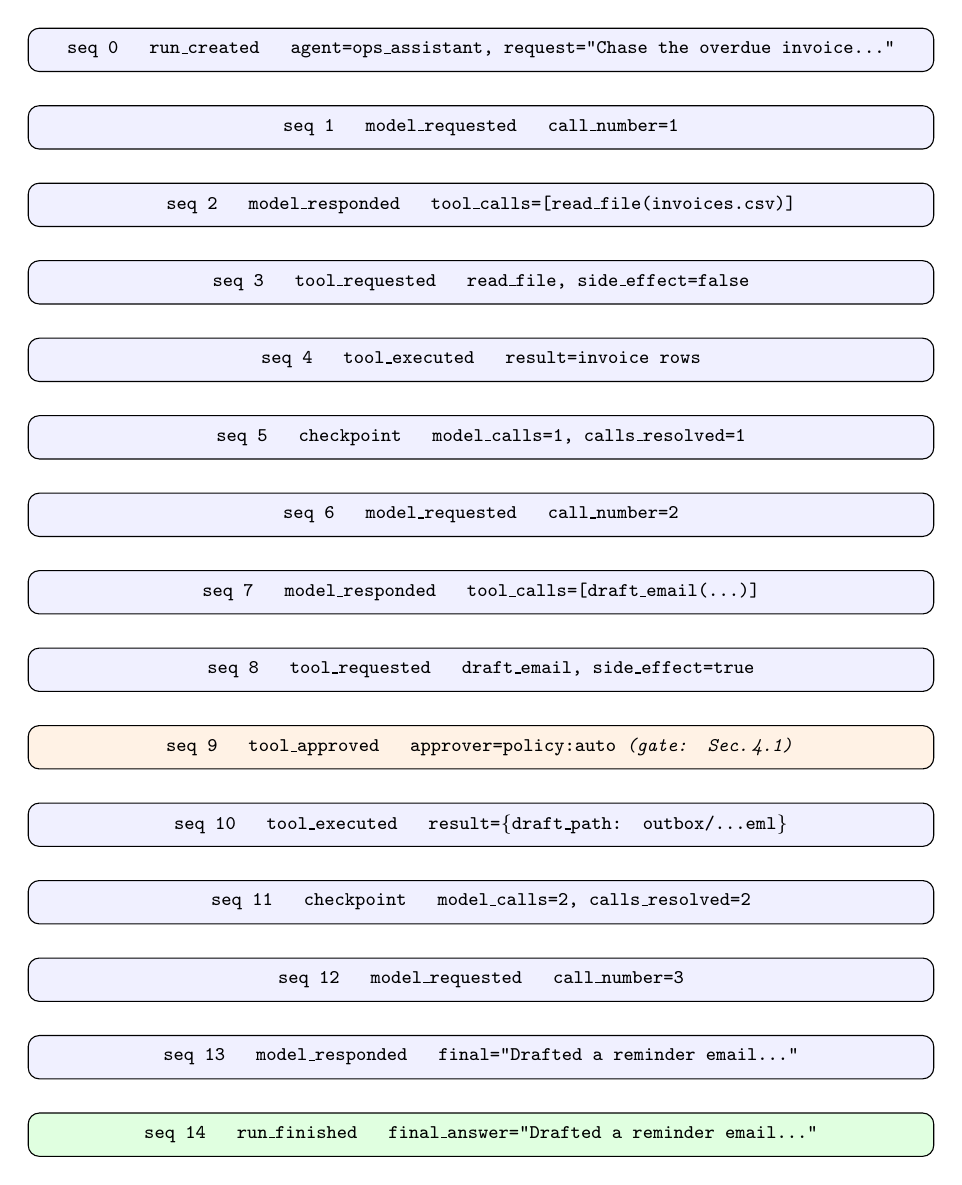
\begin{tikzpicture}[
  node distance=0.42cm and 0,
  ev/.style={draw, rounded corners, fill=blue!6, align=left, font=\scriptsize\ttfamily, minimum width=11.5cm, minimum height=0.55cm, inner sep=4pt},
  gap/.style={ev, fill=orange!10}
]
  \node[ev] (e0) {seq 0 \ \ run\_created \ \ agent=ops\_assistant, request="Chase the overdue invoice..."};
  \node[ev, below=of e0] (e1) {seq 1 \ \ model\_requested \ \ call\_number=1};
  \node[ev, below=of e1] (e2) {seq 2 \ \ model\_responded \ \ tool\_calls=[read\_file(invoices.csv)]};
  \node[ev, below=of e2] (e3) {seq 3 \ \ tool\_requested \ \ read\_file, side\_effect=false};
  \node[ev, below=of e3] (e4) {seq 4 \ \ tool\_executed \ \ result=invoice rows};
  \node[ev, below=of e4] (e5) {seq 5 \ \ checkpoint \ \ model\_calls=1, calls\_resolved=1};
  \node[ev, below=of e5] (e6) {seq 6 \ \ model\_requested \ \ call\_number=2};
  \node[ev, below=of e6] (e7) {seq 7 \ \ model\_responded \ \ tool\_calls=[draft\_email(...)]};
  \node[ev, below=of e7] (e8) {seq 8 \ \ tool\_requested \ \ draft\_email, side\_effect=true};
  \node[gap, below=of e8] (e9) {seq 9 \ \ tool\_approved \ \ approver=policy:auto  \emph{(gate: Sec.\,4.1)}};
  \node[ev, below=of e9] (e10) {seq 10 \ \ tool\_executed \ \ result=\{draft\_path: outbox/...eml\}};
  \node[ev, below=of e10] (e11) {seq 11 \ \ checkpoint \ \ model\_calls=2, calls\_resolved=2};
  \node[ev, below=of e11] (e12) {seq 12 \ \ model\_requested \ \ call\_number=3};
  \node[ev, below=of e12] (e13) {seq 13 \ \ model\_responded \ \ final="Drafted a reminder email..."};
  \node[ev, below=of e13, fill=green!12] (e14) {seq 14 \ \ run\_finished \ \ final\_answer="Drafted a reminder email..."};
\end{tikzpicture}
\end{center}

With the CLI's default auto-approve policy, \code{tool\_approved} happens
automatically at seq 9; run without \code{--auto-approve} and no policy at all, the
loop would instead stop and return \code{waiting\_approval} right before seq 9,
and a human would run \code{agentrun approvals approve <run-id> call-2-0} to
produce exactly that event and let the loop continue --- the same downstream events
(10 through 14) follow either way, because they are computed from the log, not from
which code path triggered the approval.

% ============================================================
\section{Scenario regression testing}
% ============================================================

\begin{defterm}{Regression test}
A test that exists specifically to catch a case where something that used to work
now behaves differently, typically run after a change (here: after a model version
or prompt changes) to prove nothing that used to pass now fails.
\end{defterm}

Each scenario YAML (\code{scenarios/loader.py}, validated against a strict JSON
schema) has: a \code{name}, an \code{agent}, a \code{request}, optional
\code{workspace\_files} (fixture files created before the run), one or more named
\code{behaviors} (each a full script for \code{MockModelAdapter}, Sec.\,8.1),
optional \code{approvals} (\code{auto}, or a \code{deny} list with a \code{reason}),
optional \code{faults} (Sec.\,9), and an \code{expect} block of assertions.

\subsection{Assertions}
\code{scenarios/runner.py}'s \code{check\_expectations()} evaluates every assertion
present (never short-circuiting on the first failure, so a failing scenario reports
everything wrong at once):

\begin{center}
\small
\begin{tabular}{@{}p{4.9cm}p{7.9cm}@{}}
\toprule
\textbf{Assertion key} & \textbf{Checks} \\
\midrule
\code{status} & final run status equals \code{finished}/\code{failed}/\code{waiting\_approval} \\
\code{tools\_executed} & the \emph{exact}, ordered list of tools that executed successfully \\
\code{tools\_executed\_contains} & these tools ran somewhere (order/extras ignored) \\
\code{tools\_not\_executed} & these tools never ran \\
\code{denied\_tools} & these tools were denied at the approval gate \\
\code{final\_contains} / \code{final\_not\_contains} & case-insensitive substring checks on the final answer \\
\code{failure\_cause\_contains} & substring of the recorded failure cause \\
\code{files\_exist} & workspace-relative paths that must exist afterward \\
\code{min\_events} & minimum total event count \\
\code{no\_side\_effect\_before\_approval} & every executed side-effecting call had a \code{tool\_approved} event \emph{before} its \code{tool\_executed} event, by sequence number \\
\bottomrule
\end{tabular}
\end{center}

\subsection{Running and comparing versions}
\code{agentrun test scenarios/ --behavior v1 --compare v2 --html report.html} runs
every scenario in the pack against behavior \code{v1}, then again against
\code{v2}, and diffs them. The diff mechanism
(\code{scenarios/runner.event\_signature()}) reduces each event to a compact
\code{"type:tool-or-call-id"} string (e.g.\ \code{tool\_requested:read\_file}); two
scenarios' signature lists are compared element-by-element, and the first index
where they differ is reported as the first point of behavioral divergence --- e.g.\
``expected \code{tool\_requested:read\_file}, got
\code{tool\_requested:draft\_email} at event 3.'' No general-purpose diff library is
used; a list of short strings compared position-by-position is sufficient
(\code{scenarios/report.py}'s \code{diff\_results()}). \code{terminal\_report},
\code{terminal\_diff} and \code{html\_report} render this to the console and to a
static HTML file respectively; the HTML report is generated by hand-built string
templates, not a templating library.

% ============================================================
\section{The command-line interface}
% ============================================================

\code{cli.py} exposes a single \code{agentrun} entry point (registered via
\code{pyproject.toml}'s \code{[project.scripts]}) built with \textbf{Click}, a
Python library for building command-line tools out of decorated functions.

\begin{center}
\small
\begin{tabular}{@{}p{4.6cm}p{8.2cm}@{}}
\toprule
\textbf{Command} & \textbf{What it does} \\
\midrule
\code{agentrun run --scenario \dots} & starts a mock-adapter run scripted by a scenario file; \code{--auto-approve} skips the human gate \\
\code{agentrun resume <run-id>} & rebuilds the exact runtime for an existing run from its \code{run\_created} metadata and drives it forward (Sec.\,15) \\
\code{agentrun replay <run-id> [--until N]} & deterministic replay (Sec.\,7); exits nonzero if not byte-identical \\
\code{agentrun runs list} / \code{show} & lists all runs with status/cost, or prints one run's full canonical event log \\
\code{agentrun approvals list} / \code{approve} / \code{deny} & manage the human approval queue \\
\code{agentrun test <pack> [--behavior --compare --html]} & runs the scenario regression suite (Sec.\,12) \\
\code{agentrun serve [--host --port]} & serves the FastAPI web UI (Sec.\,14) via \code{uvicorn} \\
\code{agentrun agents} & lists the built-in agent definitions and their tools \\
\bottomrule
\end{tabular}
\end{center}

Every command takes a \code{--db} option (default \code{agentrun.db}, overridable by
the \code{AGENTRUN\_DB} environment variable) pointing at the SQLite file to use.

% ============================================================
\section{The web UI}
% ============================================================

\code{web/app.py} builds a small \textbf{FastAPI} application (a Python web
framework for building HTTP APIs, here used to serve plain HTML pages instead) with
three routes:

\begin{itemize}[nosep]
  \item \code{GET /} --- a table of every run: id, agent, status badge, event count,
  cost.
  \item \code{GET /runs/\{run\_id\}} --- one run's status, cost/latency summary, any
  \emph{pending approvals} rendered as a human-readable \textbf{diff-style preview}
  of what the action would change (Sec.\,14.1), and the full event timeline.
  \item \code{POST /runs/\{run\_id\}/calls/\{call\_id\}/approve} and
  \code{/deny} --- record the decision, then call \code{resume\_run()}
  (Sec.\,15) \emph{synchronously, inside the HTTP request handler}, before
  redirecting back to the run page.
\end{itemize}

\begin{tcolorbox}[colback=red!6,colframe=red!50!black,title={Known limitation (from the README, stated by the project itself)},fonttitle=\bfseries\small]
``Approvals via the web UI resume the run synchronously inside the request handler.
A slow tool blocks the HTTP worker for its whole timeout. A real deployment needs a
worker process consuming a resume queue, with the UI only appending decision
events.''
\end{tcolorbox}

\subsection{Diff-style previews}
\code{web/preview.py}'s \code{preview(tool, args, workspace)} renders, for a
\emph{pending} side-effecting call, what it would change, before a human approves it:
for \code{write\_file} and \code{csv\_update} it computes a real unified diff
(Python's \code{difflib.unified\_diff}) between the current file content and what the
call would produce; for \code{draft\_email} and \code{calendar\_add} (which have no
natural ``before'' state to diff against) it renders a plain \code{+}-prefixed
summary of the new content instead.

\begin{defterm}{Unified diff}
A standard, compact way to show the difference between two versions of a text file:
unchanged lines shown plainly, removed lines prefixed \code{-}, added lines prefixed
\code{+}. The format produced by \code{git diff} and Unix \code{diff -u}.
\end{defterm}

% ============================================================
\section{Bootstrap: constructing runtimes for new and existing runs}
% ============================================================

\code{bootstrap.py} is the module the CLI and web UI both call into so that
``build me a working \code{Runtime} for this run'' is written exactly once. Its key
insight, stated in its own docstring: \emph{run metadata (workspace path, adapter
kind, scenario file, behavior version) lives in the \code{run\_created} event, so
any process with the database can rebuild the exact runtime needed to continue a
run} --- no separate session state has to survive a process restart.

\code{resume\_run(store, run\_id, approval\_policy)}:
\begin{enumerate}[nosep]
  \item Projects the log; if the run is already terminal, returns immediately.
  \item Counts how many \code{model\_responded} events were \emph{not} malformed
  --- this is exactly how many script turns the mock adapter has consumed, so the
  rebuilt \code{MockModelAdapter}'s \code{script\_i} is repositioned to that count.
  \item Separately counts every \code{model\_responded} \emph{or} \code{model\_error}
  event --- this is how many times \code{complete()} was called in total, used to
  reposition the mock adapter's \code{calls} counter so fault matching
  (\code{at\_call}, Sec.\,9) stays aligned after a resume.
  \item Calls \code{Runtime.drive(run\_id)}, which picks up exactly where the fixed
  point iteration (Sec.\,4) left off.
\end{enumerate}

\begin{tcolorbox}[colback=red!6,colframe=red!50!black,title={Known limitation (from the README, stated by the project itself)},fonttitle=\bfseries\small]
``Resume repositions the mock adapter by counting events. It is correct for the
states the tests cover, but a run resumed in the middle of an injected model-fault
sequence could realign fault triggers off by one. The honest fix is recording the
adapter cursor in a checkpoint payload instead of inferring it.''
\end{tcolorbox}

% ============================================================
\section{Package map}
% ============================================================

\begin{center}
\begin{forest}
for tree={
  font=\ttfamily\small, grow'=0, edge={-{Stealth[length=1.8mm]}},
  l sep=16pt, s sep=5pt, anchor=west, child anchor=west,
  parent anchor=south, calign=first,
  edge path={\noexpand\path[\forestoption{edge}] (!u.south west) +(7pt,0) |- (.child anchor)\forestoption{edge label};},
  fit=band,
  before typesetting nodes={
    if n=1{insert before={[,phantom]}}{}
  },
}
[src/agent\_runtime/
  [events.py \textnormal{\scriptsize\ttfamily\ event types + canonical JSON encoding}]
  [store.py \textnormal{\scriptsize\ttfamily\ SQLite append-only store + idempotency ledger}]
  [projection.py \textnormal{\scriptsize\ttfamily\ log $\to$ RunState, log $\to$ messages}]
  [runtime.py \textnormal{\scriptsize\ttfamily\ the loop, approval gating}]
  [replay.py \textnormal{\scriptsize\ttfamily\ recorded stand-ins + comparator}]
  [faults.py \textnormal{\scriptsize\ttfamily\ fault plans}]
  [accounting.py \textnormal{\scriptsize\ttfamily\ usage $\to$ cost/latency}]
  [agents.py \textnormal{\scriptsize\ttfamily\ example agent definitions}]
  [bootstrap.py \textnormal{\scriptsize\ttfamily\ build runtimes for new/existing runs}]
  [cli.py \textnormal{\scriptsize\ttfamily\ agentrun entry point}]
  [adapters/
    [base.py \textnormal{\scriptsize\ttfamily\ ModelAdapter interface, Turn/Usage}]
    [mock.py \textnormal{\scriptsize\ttfamily\ scripted offline adapter}]
    [anthropic\_adapter.py]
    [openai\_adapter.py]
  ]
  [tools/
    [registry.py \textnormal{\scriptsize\ttfamily\ ToolSpec, ToolRegistry, sandboxing}]
    [executor.py \textnormal{\scriptsize\ttfamily\ timeout, retries, idempotency}]
    [builtin.py \textnormal{\scriptsize\ttfamily\ the 7 shipped tools}]
  ]
  [scenarios/
    [loader.py \textnormal{\scriptsize\ttfamily\ YAML schema + loading}]
    [runner.py \textnormal{\scriptsize\ttfamily\ run one scenario, check assertions}]
    [report.py \textnormal{\scriptsize\ttfamily\ terminal + HTML reports, diffing}]
  ]
  [web/
    [app.py \textnormal{\scriptsize\ttfamily\ FastAPI timeline + approval UI}]
    [preview.py \textnormal{\scriptsize\ttfamily\ diff-style previews}]
  ]
]
\end{forest}
\end{center}

Alongside \code{src/}, the repository root has \code{scenarios/} (24 YAML fixture
files, three subfolders by agent), \code{tests/} (13 test modules, 1{,}357 lines,
93 test functions --- counted directly from the files present), \code{docs/}
(\code{ARCHITECTURE.md}, \code{WRITING\_SCENARIOS.md}), plus the standard
\code{README.md}, \code{LICENSE} (MIT), \code{pyproject.toml},
\code{requirements.txt} and \code{.env.example}.

% ============================================================
\section{Dependencies}
% ============================================================

From \code{pyproject.toml} (runtime) and the \code{dev} extra:

\begin{center}
\small
\begin{tabular}{@{}p{3.2cm}p{9.6cm}@{}}
\toprule
\textbf{Package} & \textbf{Role in this project} \\
\midrule
\code{click} & builds the \code{agentrun} CLI \\
\code{PyYAML} & parses scenario \code{.yaml} files \\
\code{jsonschema} & validates tool arguments and scenario file structure against JSON Schema \\
\code{httpx} & the HTTP client used by the live adapters and the \code{http\_get} tool \\
\code{fastapi} + \code{uvicorn} & the web UI and its ASGI server \\
\code{python-multipart} & required by FastAPI to parse the deny form's \code{reason} field (see the README's account of the one real bug this caused, below) \\
\code{pytest} (dev only) & the test suite \\
\bottomrule
\end{tabular}
\end{center}

\begin{tcolorbox}[colback=blue!6,colframe=accent,title={A real bug the project's own history records},fonttitle=\bfseries\small]
From the README: ``The first full-suite run failed with 5 errors in the web tests
only: FastAPI's \code{Form} parsing needs \code{python-multipart}, which nothing
else imports, so every non-web test passed and the gap only surfaced when the
deny-with-reason endpoint was exercised through \code{TestClient}. Pinned it as a
real dependency rather than a test extra since the deny form is a runtime feature.''
This is reflected in \code{pyproject.toml}, where \code{python-multipart} is listed
as a core dependency, not under \code{dev}.
\end{tcolorbox}

% ============================================================
\section{Testing}
% ============================================================

The test suite (\code{tests/}, run with \code{pytest}) has 93 test functions across
13 files (counted directly: \code{test\_accounting.py}, \code{test\_adapters.py},
\code{test\_cli.py}, \code{test\_executor.py}, \code{test\_faults.py},
\code{test\_replay.py}, \code{test\_resume.py}, \code{test\_runtime.py},
\code{test\_scenarios.py}, \code{test\_store.py}, \code{test\_tools.py},
\code{test\_web.py}, plus shared fixtures in \code{conftest.py}), matching the
count the README states (``93 tests, all offline''). \code{conftest.py} provides a
\code{make\_runtime()} helper that wires a fresh in-memory-style SQLite store, a
sandbox workspace, the mock adapter and an auto-approve policy with a single call,
used throughout the other test files. Every test runs offline: no test in this
repository makes a live network call to Anthropic or OpenAI.

% ============================================================
\section{What the project's own retrospective says}
% ============================================================

The README includes a ``What I learned'' and ``What I'd do differently'' section
written by the project's author. Reproduced here verbatim (not paraphrased, so
nothing is lost or oversold) because it is part of the project's own honest account
of its design and limits:

\subsection*{What was learned}
\begin{itemize}[nosep]
  \item Deriving all state from a projection collapsed the feature count: resume
  after crash, continue after approval, and a plain next loop iteration became
  literally the same function, so the recovery tests exercise the normal path
  rather than a bespoke one.
  \item Determinism is a budget spent field by field: any payload value that is not
  a pure function of the log (a timestamp, a real-sleep-dependent attempt count, a
  random id) is a future replay divergence.
  \item Separating expected tool failures (\code{ToolError}) from unexpected ones
  buys a retry policy for free: deterministic refusals fail fast, transient
  exceptions and timeouts consume the retry budget with backoff.
  \item \code{concurrent.futures} timeouts abandon the worker thread rather than
  kill it --- a timeout answers ``how long do I wait,'' not ``how do I stop the
  tool.'' Documented rather than papered over.
  \item A per-event \code{"type:detail"} signature is enough for useful regression
  diffs, with no diffing library needed.
\end{itemize}

\subsection*{What the author would do differently}
\begin{itemize}[nosep]
  \item The web UI's synchronous approval-resume should become a worker process
  consuming a resume queue.
  \item Resume's event-counting approach to repositioning the mock adapter is
  correct for tested states but could misalign fault triggers in an edge case; a
  recorded adapter cursor in the checkpoint payload would be the honest fix.
  \item Event payloads carry no schema version; replay currently detects divergence
  as a tripwire, not a migration story.
  \item Tool timeouts do not kill the handler thread, so a truly hung tool leaks a
  thread per attempt; subprocess isolation would fix this and give tools their own
  memory space.
  \item The in-house neutral message format ignores streaming and
  provider-specific parallel tool-call semantics; the accounting price table is
  hardcoded and will drift.
\end{itemize}

% ============================================================
\section{Glossary}
% ============================================================
\begin{description}[leftmargin=3.4cm, style=nextline]
\item[Agent] A program that uses an LLM in a loop to decide and take actions via tools.
\item[Adapter] A class implementing a fixed interface around a specific model API or fake.
\item[Allowlist] A set of explicitly permitted values; everything else is rejected.
\item[Approval gate] The point in the loop where a side-effecting tool call pauses for a human decision.
\item[Backoff] Waiting longer between each successive retry.
\item[Canonical encoding] A deterministic serialization where equal data always produces an identical string.
\item[Checkpoint] A periodic event recording loop progress, for readability, not correctness.
\item[Contract test] A test verifying request/response shape against a real API's spec, without calling the real API.
\item[Digest / hash] A short fixed-length fingerprint of a larger piece of data.
\item[Event sourcing] Storing every state change as an immutable ordered log instead of overwriting current state.
\item[Fixed-point iteration] A loop that recomputes its next step purely from its own last output.
\item[Idempotency] Doing an operation twice has the same effect as doing it once.
\item[JSON Schema] A specification language describing the required shape of JSON data.
\item[LLM] Large language model: a machine learning model that generates text (or structured output) from a prompt.
\item[Primary key] A column set guaranteed unique per row, used to enforce no-duplicate writes.
\item[Projection] Computing derived state from an event log.
\item[Regression test] A test proving something that used to work still works after a change.
\item[Replay] Re-driving logic from only recorded data, with no live calls, and checking the result matches.
\item[Sandbox] A restricted environment limiting what a program can access.
\item[Side effect] An action with a lasting, observable consequence outside the program.
\item[Unified diff] A standard compact text format for showing line-level differences between two versions of a file.
\end{description}

\end{document}
